\documentclass{beamer}

\usepackage{comment}
\usepackage{color}
\usepackage{listings}
\usepackage{verbatim}
\usepackage{multicol}
\usepackage{booktabs}
\definecolor{green}{RGB}{0,128,0}

\usetheme{CambridgeUS}
\setbeamercolor*{item}{fg=red}

\def\EQ#1\EN{\begin{equation*}#1\end{equation*}}
\def\BA#1\EA{\begin{align*}#1\end{align*}}
\def\BS#1\ES{\begin{split*}#1\end{split*}}
\newcommand{\bc}{\begin{center}}
\newcommand{\ec}{\end{center}}
\newcommand{\eq}{\ =\ }
\newcommand{\degc}{$^\circ$C}

\def\p{\partial}
\def\qbs{\boldsymbol{q}}
\def\Dbs{\boldsymbol{D}}
\def\A{\mathcal A}
\def\gC{\mathcal C}
\def\gD{\mathcal D}
\def\gL{\mathcal L}
\def\M{\mathcal M}
\def\P{\mathcal P}
\def\Q{\mathcal Q}
\def\gR{\mathcal R}
\def\gS{\mathcal S}
\def\X{\mathcal X}
\def\bnabla{\boldsymbol{\nabla}}
\def\bnu{\boldsymbol{\nu}}
\renewcommand{\a}{{\alpha}}
%\renewcommand{\a}{{}}
\newcommand{\s}{{\sigma}}
\newcommand{\bq}{\boldsymbol{q}}
\newcommand{\bz}{\boldsymbol{z}}
\def\bPsi{\boldsymbol{\Psi}}

\def\Li{\textit{L}}
\def\Fb{\textbf{f}}
\def\Jb{\textbf{J}}
\def\cb{\textbf{c}}

\def\Dt{\Delta t}
\def\tpdt{{t + \Delta t}}
\def\bpsi{\boldsymbol{\psi}}
\def\dbpsi{\delta \boldsymbol{\psi}}
\def\bc{\textbf{c}}
\def\dbc{\delta \textbf{c}}
\def\arrows{\rightleftharpoons}

\newcommand{\bGamma}{\boldsymbol{\Gamma}}
\newcommand{\bOmega}{\boldsymbol{\Omega}}
%\newcommand{\bPsi}{\boldsymbol{\Psi}}
%\newcommand{\bpsi}{\boldsymbol{\psi}}
\newcommand{\bO}{\boldsymbol{O}}
%\newcommand{\bnu}{\boldsymbol{\nu}}
\newcommand{\bdS}{\boldsymbol{dS}}
\newcommand{\bg}{\boldsymbol{g}}
\newcommand{\bk}{\boldsymbol{k}}
%\newcommand{\bq}{\boldsymbol{q}}
\newcommand{\br}{\boldsymbol{r}}
\newcommand{\bR}{\boldsymbol{R}}
\newcommand{\bS}{\boldsymbol{S}}
\newcommand{\bu}{\boldsymbol{u}}
\newcommand{\bv}{\boldsymbol{v}}
%\newcommand{\bz}{\boldsymbol{z}}
\newcommand{\pressure}{P}

\def\water{H$_2$O}
\def\calcium{Ca$^{2+}$}
\def\copper{Cu$^{2+}$}
\def\magnesium{Mg$^{2+}$}
\def\sodium{Na$^+$}
\def\potassium{K$^+$}
\def\uranium{UO$_2^{2+}$}
\def\hion{H$^+$}
\def\bicarbonate{HCO$_3^-$}
\def\cotwo{CO$_2$}
\def\chloride{Cl$^-$}
\def\fluoride{F$^-$}
\def\phosphoricacid{HPO$_4^{2-}$}
\def\nitrate{NO$_3^-$}
\def\sulfate{SO$_4^{2-}$}
\def\souotwooh{$>$SOUO$_2$OH}
\def\sohuotwocothree{$>$SOHUO$_2$CO$_3$}
\def\soh{$>$SOH}

\newcommand\gehcomment[1]{{{\color{orange} #1}}}
\newcommand\add[1]{{{\color{blue} #1}}}
\newcommand\remove[1]{\sout{{\color{red} #1}}}
\newcommand\codecomment[1]{{{\color{green} #1}}}
\newcommand\redcomment[1]{{{\color{red} #1}}}
\newcommand\bluecomment[1]{{{\color{blue} #1}}}
\newcommand\greencomment[1]{{{\color{green} #1}}}

\begin{comment}
\tiny
\scriptsize
\footnotesize
\small
\normalsize
\large
\Large
\LARGE
\huge
\Huge
\end{comment}

\begin{document}
\title{PFLOTRAN Input Cards}
\author{Glenn Hammond}
\date{\today}

\frame{\titlepage}


\section{Syntax}

\begin{frame}[containsverbatim]\frametitle{Syntax}

The PFLOTRAN input deck is defined using keywords or cards that are associated with data.  The file is designed with modularity in mind and the cards need not be in any particular order.  Many cards open a section that provides additional cards and is terminated by an ``END'' or ``/''.  For example:

\begin{semiverbatim}
CARD1
  CARD2 value value
  CARD3
    CARD4 value
    CARD5 value
  /
END
\end{semiverbatim}

\end{frame}

\begin{frame}[fragile]\frametitle{Syntax (cont.)}
Several options exist for commenting out lines or sections of the input file:
\begin{itemize}
\item Individual lines may be commented out by placing a colon (:) or exclamation point (!) at the beginning of line (i.e. before any text).
\item The SKIP/NOSKIP cards may be used to comment out a large number of lines.  SKIP/NOSKIP may be used in a nested manner.  But beware!  One must ensure consistency (i.e. \# SKIPs == \# NOSKIPs).
\item Exclamation points (!) are often used to place comments at the end of a line, but serve no purpose and are solely for markup (i.e. PFLOTRAN will continue to read the string if it is expecting additional entry data).
\end{itemize}

\end{frame}


\section{BOUNDARY\_CONDITION Card}

\begin{frame}[fragile,containsverbatim]\frametitle{BOUNDARY\_CONDITION}

\begin{itemize}
\item[] \textbf{Purpose:} Couples a flow and/or transport conditions with a region to create a boundary condition.
\item[] \textbf{Example uses:}
\begin{itemize}
  \item To assign a boundary condition
\end{itemize}
\end{itemize}

\end{frame}

\begin{frame}[fragile]\frametitle{BOUNDARY\_CONDITION: Examples}

\begin{semiverbatim}
\scriptsize
: west boundary condition
BOUNDARY_CONDITION
  FLOW_CONDITION initial
  TRANSPORT_CONDITION west
  REGION West
END

: east boundary condition
BOUNDARY_CONDITION
  FLOW_CONDITION initial
  TRANSPORT_CONDITION initial
  REGION East
END

\end{semiverbatim}


\end{frame}

\section{CHECKPOINT Card}

\begin{frame}[fragile,containsverbatim]\frametitle{CHECKPOINT}

\begin{itemize}{}
\item[] \textbf{Purpose:} Toggle on checkpoint/restart capability and specifies the frequency at which checkpoint files are created.  A restart file is created when the simulation terminates as scheduled.

\item[] \textbf{Example uses:}
\begin{itemize}
\item Save the state of a simulation every 100 time steps
\item Save the state of a simulation once the final time has been reached.  
\item Fault tolerance
\end{itemize}
\end{itemize}

\end{frame}



\section{CHEMISTRY Card}

\begin{frame}[fragile,containsverbatim]\frametitle{CHEMISTRY}

\begin{itemize}
\item[] \textbf{Purpose:} Defines basis species and all chemical reactions based on those species.  Also defines output options for reactive transport.
\item[] \textbf{Example uses:}
\begin{itemize}
  \item Naming chemistry components
  \item Defining geochemistry:
    \begin{itemize}
      \item Defining basis species
      \item Aqueous speciation reactions
      \item Minerals and mineral reactions
      \item Activity calculations
      \item Database name
    \end{itemize}
\end{itemize}
\end{itemize}

\end{frame}

\begin{frame}[fragile]\frametitle{CHEMISTRY: Examples}

\end{frame}

\section{CONSTRAINT Card}

\begin{frame}[fragile,containsverbatim]\frametitle{CONSTRAINT}

\begin{itemize}
\item[] \textbf{Purpose:} Defines a set of concentrations for the primary or basis species (and potentially minerals) to be referenced by a transport condition.
\item[] \textbf{Example uses:}
\begin{itemize}
  \item Defining free-ion or total component concentrations of primary species
  \item Equilibrating species concentrations with a mineral such as Calcite
  \item Defining mineral volume fractions
  \item Setting a species concentration based on charge balance
\end{itemize}
\end{itemize}

\end{frame}

\begin{frame}[fragile]\frametitle{CONSTRAINT: Examples}

\end{frame}

\section{Coupler}

\begin{frame}[fragile,containsverbatim]\frametitle{PFLOTRAN Coupler}

\begin{itemize}
\item[] \textbf{Purpose:} Couples a flow and/or transport conditions with a region to create a boundary condition, initial condition or source/sink.
\item[] \textbf{Example uses:}
\begin{itemize}
  \item Assign a boundary condition to a face of the model
  \item Assign initial concentrations to a zone in the model
  \item Assign an injection well with in the model domain
\end{itemize}
\end{itemize}
\end{frame}

\begin{frame}[fragile,containsverbatim]\frametitle{PFLOTRAN Coupler}
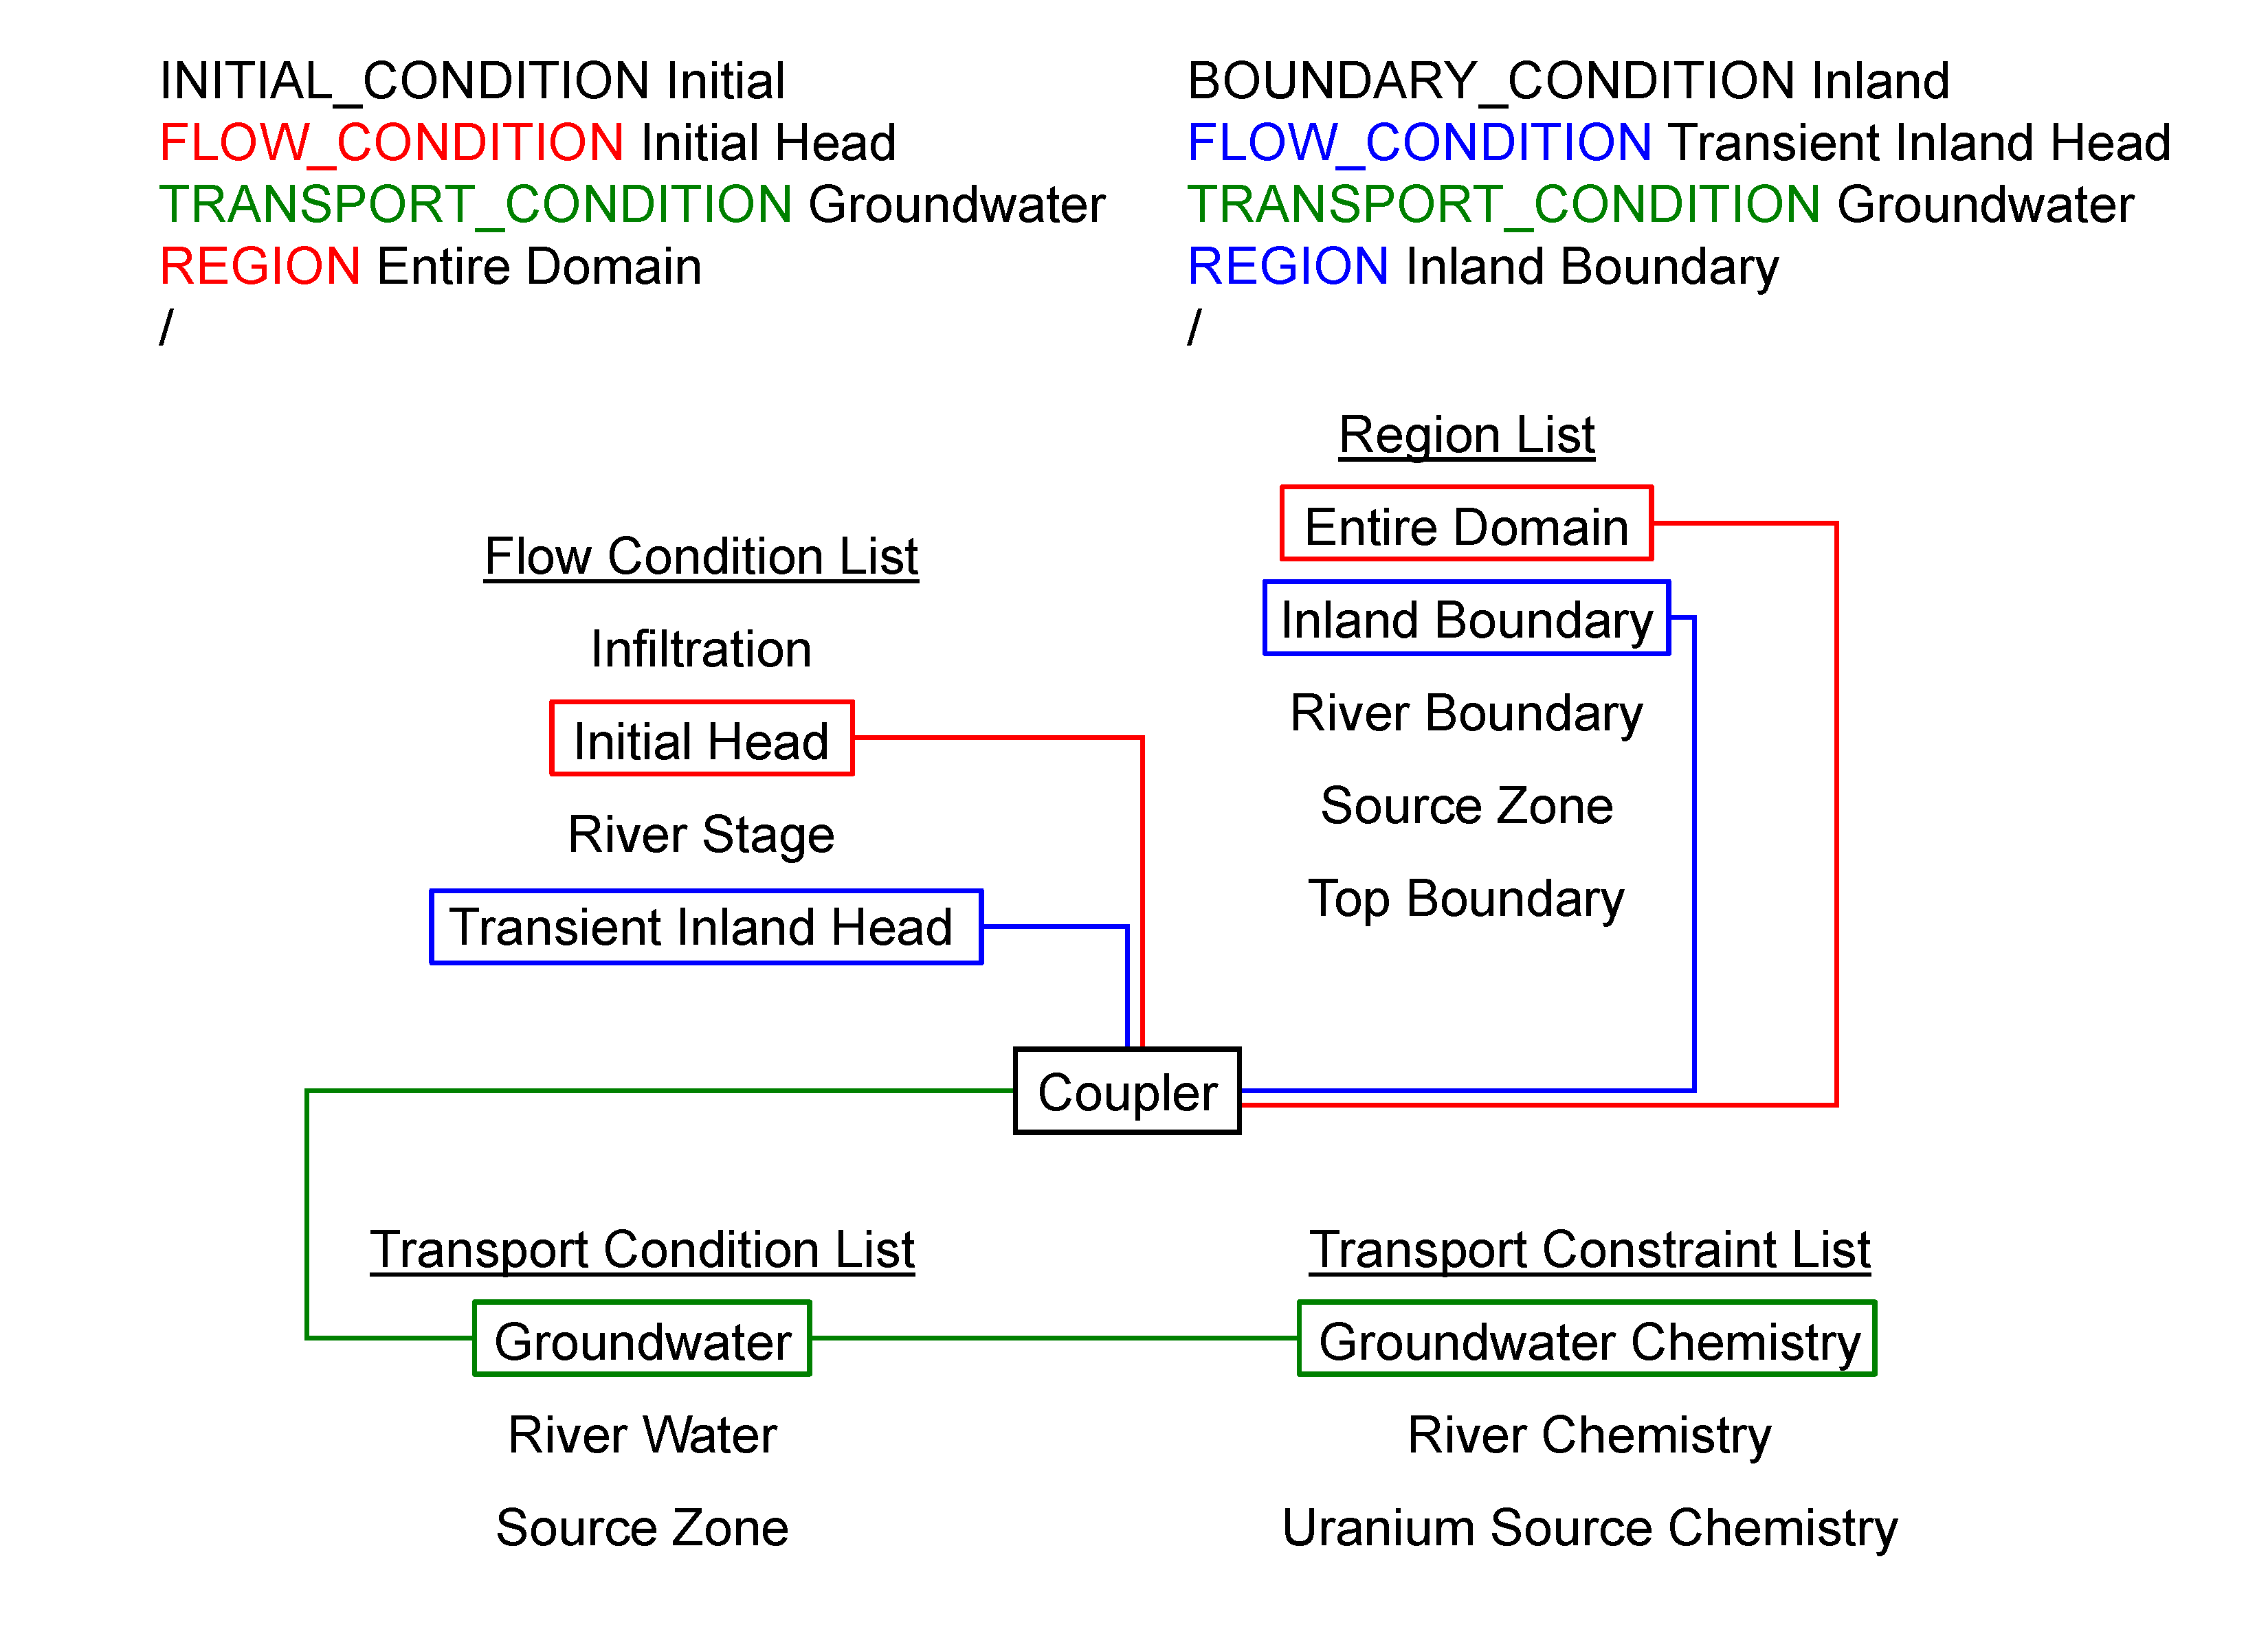
\includegraphics[width=\linewidth]{coupler.pdf}
\end{frame}

[suites]
standard = top_surface_node_centered
           top_surface_cell_centered
           east_surface_node_centered
           east_surface_cell_centered
           north_surface_node_centered
           north_surface_cell_centered
           x_line_node_centered
           x_line_cell_centered
           y_line_node_centered
           y_line_cell_centered
           z_line_node_centered
           z_line_cell_centered

[default-test-criteria]
# default criteria for all tests, can be overwritten by specific tests
time = 500 percent
generic = 1.0e-12 absolute
concentration = 1.0e-9 relative
discrete = 0 absolute
rate = 1.0e-12 absolute
volume_fraction = 1.0e-12 absolute
pressure = 1.0e-12 relative
saturation = 1.0e-12 absolute

[top_surface_node_centered]

[top_surface_cell_centered]

[east_surface_node_centered]

[east_surface_cell_centered]

[north_surface_node_centered]

[north_surface_cell_centered]

[x_line_node_centered]

[x_line_cell_centered]

[y_line_node_centered]

[y_line_cell_centered]

[z_line_node_centered]

[z_line_cell_centered]


\section{DEBUG Card}

\begin{frame}[fragile,containsverbatim]\frametitle{DEBUG}

\begin{itemize}{}
\item[] \textbf{Purpose:} A list of toggles for turning on the writing of vectors and matrices for debugging purposes.

\item[] \textbf{Example uses:}
\begin{itemize}
\item Print the Jacobian
\item Print the residual vector
\end{itemize}
\end{itemize}

\end{frame}



\section{FLOW\_CONDITION Card}

\begin{frame}[fragile,containsverbatim]\frametitle{FLOW\_CONDITION}

\begin{itemize}
\item[] \textbf{Purpose:} To specify a fluid pressure, saturation, or flux to be associated with a flow boundary/initial condition or source/sink
\item[] \textbf{Example uses:}
\begin{itemize}
  \item Assigning a pressure to the vertical boundary of a model
  \item Assigning a flux to a boundary face (e.g. recharge)
  \item Assigning an initial saturation in the model domain (to be implemented)
  \item Assigning an initial hydrostatic pressure distribution in a model domain
  \item Assigning an injection rate for a well
\end{itemize}
\end{itemize}

\end{frame}

\begin{frame}[fragile]\frametitle{FLOW\_CONDITION: Examples}

\begin{semiverbatim}
\scriptsize

\end{semiverbatim}


\end{frame}

\section{FLUID\_PROPERTY Card}

\begin{frame}[fragile,containsverbatim]\frametitle{FLUID\_PROPERTY}

\begin{itemize}
\item[] \textbf{Purpose:} Define fluid properties
\item[] \textbf{Example uses:}
\begin{itemize}
  \item Assigning a coefficient of diffusion
\end{itemize}
\end{itemize}

\end{frame}

\begin{frame}[fragile]\frametitle{FLUID\_PROPERTY: Examples}

\end{frame}

\section{GRID Card}

\begin{frame}[fragile,containsverbatim]\frametitle{GRID}

\begin{itemize}
\item[] \textbf{Purpose:} Defines the type of grid/mesh to be employed and parameters describing the grid
\item[] \textbf{Example uses:}
\begin{itemize}
  \item Defining a structured AMR grid
  \item Defining the bounding box and resolution of a structured grid
  \item Defining the origin of a grid
\end{itemize}
\end{itemize}

\end{frame}

\begin{frame}[fragile]\frametitle{GRID: Examples}

\end{frame}

\section{INITIAL\_CONDITION Card}

\begin{frame}[fragile,containsverbatim]\frametitle{INITIAL\_CONDITION}

\begin{itemize}
\item[] \textbf{Purpose:} Couples a flow and/or transport conditions with a region to create an initial condition.
\item[] \textbf{Example uses:}
\begin{itemize}
  \item To assign a initial condition.
\end{itemize}
\end{itemize}

\end{frame}

\begin{frame}[fragile]\frametitle{INITIAL\_CONDITION: Examples}

\end{frame}

\section{LINEAR\_SOLVER Card}

\begin{frame}[fragile,containsverbatim]\frametitle{LINEAR\_SOLVER}

\begin{itemize}
\item[] \textbf{Purpose:} Defines the linear solver and preconditioner to be employed and linear solver convergence criteria
\item[] \textbf{Example uses:}
\begin{itemize}
  \item Assigning a direct solver (e.g. LU)
  \item Assigning a Krylov solver (e.g. BiCGSTAB)
  \item Assigning a preconditioner (e.g. block Jacobi, ILU[0])
  \item Defining linear solver convergence criteria
  \item Defining pivoting tolerances for LU/ILU
\end{itemize}
\end{itemize}

\end{frame}

\begin{frame}[fragile]\frametitle{LINEAR\_SOLVER: Examples}

\end{frame}

\section{MATERIAL\_PROPERTY Card}

\begin{frame}[fragile,containsverbatim]\frametitle{MATERIAL\_PROPERTY}

\begin{itemize}
\item[] \textbf{Purpose:} Defines parameters/properties associated with subsurface soil/rock.
\item[] \textbf{Example uses:}
\begin{itemize}
  \item Assigning permeability of the soil/rock formation
  \item Assigning porosity
  \item Coupling a material type with a permeability/saturation function
\end{itemize}
\end{itemize}

\end{frame}

\begin{frame}[fragile]\frametitle{MATERIAL\_PROPERTY: Examples}

\end{frame}

\section{MODE Card}

\begin{frame}[fragile,containsverbatim]\frametitle{MODE}

\begin{itemize}{}
\item[] \textbf{Purpose:} Declares the flow mode


\item[] \textbf{Examples:}
\end{itemize}

\end{frame}



\section{NEWTON\_SOLVER Card}

\begin{frame}[fragile,containsverbatim]\frametitle{NEWTON\_SOLVER}

\begin{itemize}
\item[] \textbf{Purpose:} Declares parameters associated with the nonlinear solve
\item[] \textbf{Example uses:}
\begin{itemize}
  \item Defining convergence tolerances
  \item Defining level of detail regarding printed convergence information
  \item Defining maximum number of Newton iterations before cutting time step size
  \item Defining Jacobian matrix format (e.g. AIJ vs. BAIJ)
\end{itemize}
\end{itemize}

\end{frame}

\begin{frame}[fragile]\frametitle{NEWTON\_SOLVER: Examples}

\end{frame}

\section{OUTPUT Card}

\begin{frame}[fragile,containsverbatim]\frametitle{OUTPUT}

\begin{itemize}
\item[] \textbf{Purpose:} Defines output parameters such as output times, output frequency, file formats, advanced output (e.g. mass balance calculations, observation points)
\item[] \textbf{Example uses:}
\begin{itemize}
  \item Setting the output frequency to every 100 time steps
  \item Requesting output at 100.5 years
  \item Requesting both ASCII and binary HDF5 formats
  \item Differentiating between Tecplot point versus block formats
\end{itemize}
\end{itemize}

\end{frame}

\begin{frame}[fragile]\frametitle{OUTPUT: Examples}

\end{frame}

\section{REGION Card}

\begin{frame}[fragile,containsverbatim]\frametitle{REGION}

\begin{itemize}{}
\item[] \textbf{Purpose:} To define a region within the model domain to be associated with another entity within the simulation.
\item[] \textbf{Example uses:}
\begin{itemize}
  \item To assign a recharge boundary condition to the top surface of the model
  \item To assign material properties to a zone in the model
  \item To assign a source/sink term representing an injection well to cells intercepted by the well string
  \item To an initial condition to a zone in the model
\end{itemize}
\end{itemize}

\end{frame}


\begin{frame}[fragile]\frametitle{REGION: Examples}

\scriptsize
\begin{multicols}{2}

\textbf{Volume:}
\begin{semiverbatim}
REGION all
  COORDINATES
    0. 0. 0.
    100. 100. 10.
  /
/
\end{semiverbatim}
\textbf{Surface:}
\begin{semiverbatim}
REGION river
  COORDINATES
    0. 0. 0.
    0. 100. 10.
  /
  FACE west
/
\end{semiverbatim}

\textbf{Surface:}
\begin{semiverbatim}
REGION river
  BLOCK 1 1 1 100 1 10
  FACE west
/
\end{semiverbatim}

\textbf{Point:}
\begin{semiverbatim}
REGION observation_point
  COORDINATE 50. 50. 5.
/
\end{semiverbatim}

\textbf{List of cells and faces:}
\begin{semiverbatim}
REGION FILE river.h5
\end{semiverbatim}


\end{multicols}

\end{frame}

\section{RESTART Card}

\begin{frame}[fragile,containsverbatim]\frametitle{RESTART}

\begin{itemize}{}
\item[] \textbf{Purpose:} Specifies name of restart file and time at which to restart, if different than time checkpointed in restart file.

\item[] \textbf{Example uses:}
\begin{itemize}
\item Restart a simulation from a checkpoint file.
\item Start a simulation, using a previous simulations state as the initial condition for the new simulation
\item Restart a simulation immediately prior to a segmentation fault for debugging purposes
\end{itemize}
\end{itemize}

\end{frame}



\section{SATURATION\_FUNCTION Card}

\begin{frame}[fragile,containsverbatim]\frametitle{SATURATION\_FUNCTION}

\begin{itemize}
\item[] \textbf{Purpose:} Defines parameter associated with saturation and permeability functions
\item[] \textbf{Example uses:}
\begin{itemize}
  \item Defining the air entry pressure for variable saturated flow
  \item Assigning the $\lambda$ to the Brooks-Corey relationship
  \item Assigning the permeability function type (e.g. Mualem)
\end{itemize}
\end{itemize}

\end{frame}

\begin{frame}[fragile]\frametitle{SATURATION\_FUNCTION: Examples}

\end{frame}

\section{STRATA Card}

\begin{frame}[fragile,containsverbatim]\frametitle{STRATA}

\begin{itemize}
\item[] \textbf{Purpose:} Couples a material id with a region
\item[] \textbf{Example uses:}
\begin{itemize}
  \item Assigning a material id to a region
  \item Reading in materia IDs on a cell by cell basis
\end{itemize}
\end{itemize}

\end{frame}

\begin{frame}[fragile]\frametitle{STRATA: Examples}

\end{frame}

\section{TIME Card}

\begin{frame}[fragile,containsverbatim]\frametitle{TIME}

\begin{itemize}
\item[] \textbf{Purpose:} Specifies critical times during the simulation
\item[] \textbf{Example uses:}
\begin{itemize}
  \item Defining the final time
  \item Defining initial time step size
  \item Defining maximum time step size
\end{itemize}
\end{itemize}

\end{frame}

\begin{frame}[fragile]\frametitle{TIME: Examples}

\end{frame}

\section{TIMESTEPPER Card}

\begin{frame}[fragile,containsverbatim]\frametitle{TIMESTEPPER}

\begin{itemize}
\item[] \textbf{Purpose:} Defines runtime parameters associated with time stepping
\item[] \textbf{Example uses:}
\begin{itemize}
  \item Defining maximum number of time steps
  \item Defining maximum number of consecutive time step cuts before aborting simulation
  \item Defining time step size acceleration (rate of increase in time step size)
  \item Specifying a steady state simulation
\end{itemize}
\end{itemize}

\end{frame}

\begin{frame}[fragile]\frametitle{TIMESTEPPER: Examples}

\end{frame}

\section{TRANSPORT\_CONDITION Card}

\begin{frame}[fragile,containsverbatim]\frametitle{TRANSPORT\_CONDITION}

\begin{itemize}
\item[] \textbf{Purpose:} To specify solute concentrations to be associated with a transport boundary/initial condition or source/sink
\item[] \textbf{Example uses:}
\begin{itemize}
  \item Assigning time varying concentrations at a boundary
  \item Specifying the initial species composition of the fluid
  \item Assigning a boundary condition type (e.g. Dirichlet, Neumann, zero gradient)
\end{itemize}
\end{itemize}

\end{frame}

\begin{frame}[fragile]\frametitle{TRANSPORT\_CONDITION: Examples}

\end{frame}


\section{Miscellaneous Cards}

\begin{frame}[fragile,containsverbatim]\frametitle{Miscellaneous Cards}

\begin{itemize}
\item[] REFERENCE\_DENSITY: Specifies a reference density for simulations assuming constant fluid density (e.g. solute transport only).  
\item[] REFERENCE\_PRESSURE: Specifies a reference pressure (e.g. atmospheric pressure for capillary pressure calculation)
\item[] REFERENCE\_TEMPERATURE: Specifies a reference temperature for isothermal simulations.  25\degc is the default.
\item[] UNIFORM\_VELOCITY: Specifies a velocity vector for solute transport in a uniform flow field (no flow calculation).
\item[] WALLCLOCK\_STOP: Specifies a time (in hours since the beginning of execution) at which point the simulation gracefully shuts down.  Useful in combination with the CHECKPOINT/RESTART cards for running a simulation beyond the time permitted by a given queue on a supercomputer.

\end{itemize}

\end{frame}

\begin{frame}[fragile]\frametitle{Miscellaneous Card Examples}

\end{frame}


\end{document} 